\documentclass[11pt]{article}
\usepackage[margin=1in]{geometry}
\usepackage[T1]{fontenc}
\usepackage{lmodern}
\usepackage{microtype}
\usepackage{amsmath,amssymb}
\usepackage{booktabs}
\usepackage{enumitem}
\usepackage{tikz}
\usetikzlibrary{arrows.meta,positioning,shapes.geometric,fit,calc}
\usepackage[hidelinks]{hyperref}
\usepackage{natbib}
\setcitestyle{authoryear,round}
\setlist{itemsep=2pt,topsep=4pt}
\newcommand{\pause}[1]{\langle\sigma_{#1}\rangle}
\usepackage{array}
\newcommand{\Psii}{\Psi}

\title{\textbf{MindFrame: An Inner Language for Self-Talk,\\ an Integrated Low-Overload Framework,\\ and the $\Psi$ Daily Reflection Index}\\[4pt]
\large A Combined Concept and Position Paper}
\author{Ryan Espinosa\\[2pt]
\small\url{https://github.com/ryryespi/mindframe}\quad\textbullet\quad\url{https://ryryespi.github.io/mindframe/}}
\date{October 2026}

\begin{document}
\maketitle

\begin{center}
\emph{All credit and glory to God. I owe my knowledge to my Lord Jesus Christ.}
\end{center}
\vspace{4pt}

\begin{abstract}
\noindent MindFrame is a small, static web application in which a user writes down a thought and receives four short, structured responses drawn from Dialectical Behavior Therapy (DBT), Stoic and existential philosophy, a cognitive-behavioral ``evidence worksheet,'' and self-compassion with Acceptance and Commitment Therapy (ACT) defusion. A transparent rule-based analyzer tags the text, and any crisis language bypasses every bot and shows only crisis resources. This combined paper does three things. First, it documents the prototype as it exists. Second, it proposes a broader framework: (1)~an \emph{inner language} for self-talk defined by pacing, deliberate silence, and a limited vocabulary, written as a small grammar with simple time-weighting math; (2)~an integrated self-help pipeline that helps users work constructively with grandiose ambitions and intrusive ``good or evil'' thoughts and turn them toward realistic, values-based goals and positive imagery; (3)~3D visualization of thought structures; (4)~a ``bridging layer'' between fields and plain speech, \emph{inspired by} the Langlands program as a metaphor only; and (5)~overload control grounded in cognitive load theory. Third, it introduces the \textbf{$\Psi$ daily reflection index}, $\Psi = 0.18C + 0.14S + 0.12M - 0.26R - 0.31B$, a linear combination of five 0--1 self-report terms (calm, support, skills use, avoidance, and thought believability) rescaled to a 0--100 Daily Score. We explain how $\Psi$ was derived from an earlier conceptual equation, how its weights were set by normalizing correlation magnitudes reported in published studies, and why those weights are a rough starting point. \textbf{$\Psi$ is a heuristic self-reflection aid. It is not validated and it is not a diagnosis.} We discuss safety and ethics, give a worked example with clearly labeled example values, outline an evaluation plan with no fabricated results, and end by proposing a next project, \emph{MindFrame $\Psi$-Lab}, that unites the inner-language framework with the daily index under an N-of-1 validation design.
\end{abstract}

\section{Introduction}
Most people talk to themselves. Psychologists call this \emph{inner speech}, and it has been studied since at least \citet{vygotsky1986}, who argued that children's out-loud ``private speech'' becomes silent, compressed inner speech that helps them plan and regulate behavior. Modern work finds that inner speech is common, takes different forms (dialogic, condensed, expanded), and is tied to self-regulation \citep{aldersonday2015,fernyhough2016}. The \emph{way} we address ourselves seems to matter as well: in one line of experiments, using one's own name or ``you'' instead of ``I'' during self-talk was associated with better emotion regulation under stress \citep{kross2014}.

Several well-established psychotherapies also work, in large part, by changing a person's relationship to their thoughts. Cognitive therapy teaches people to examine thoughts as hypotheses \citep{beck1979}; DBT teaches concrete skills for distress tolerance and emotion regulation \citep{linehan2015}; ACT teaches \emph{defusion}, noticing a thought as a thought \citep{hayes2012}; and self-compassion research describes a kinder stance toward one's own suffering \citep{neff2003}. Stoic philosophy, a historical influence on cognitive therapy \citep{robertson2010}, says something similar: we are disturbed not by things but by our judgments about them \citep{epictetus}.

MindFrame began as a beginner's software project built on these ideas. It is deliberately simple: a text box, a keyword analyzer, four template-based ``bots,'' and a local journal. This paper has two aims. First, it documents the prototype honestly, including where its math is a heuristic rather than a measurement. Second, it sets out a research agenda for a richer system: a small \emph{inner language} for self-talk, an integrated skills pipeline, calming 3D visualization, and an AI ``bridge'' between fields that avoids information overload.

\paragraph{Contributions.} (i)~A description of the MindFrame prototype from its source code (Section~\ref{sec:proto}); (ii)~a proposed framework of five parts (Section~\ref{sec:framework}); (iii)~the $\Psi$ daily reflection index, with its origin, measures, literature-based weights, applications, and caveats (Section~\ref{sec:psi}); (iv)~safety, ethics, and an evaluation plan (Sections~\ref{sec:safety}--\ref{sec:eval}); and (v)~a concrete next project that unites the framework with the index (Section~\ref{sec:next}).

\paragraph{A note on epistemic status.} This is a concept paper. Claims about DBT, CBT, ACT, self-compassion, inner speech, and cognitive load cite published work. The inner-language formalism, the integration pipeline, the 3D design, the Langlands-inspired bridge, and the $\Psi$ index are \textbf{proposals}. Where $\Psi$ uses numbers from published studies, those numbers are real and cited, but combining them into one formula is our own heuristic step. They have not been tested, and nothing here should be read as evidence that they help anyone.

\section{Background}
\subsection{Evidence-based skills traditions}
\textbf{CBT.} Beck's cognitive model holds that emotional distress is maintained partly by automatic, biased interpretations, and that examining evidence for and against them can reduce distress \citep{beck1976,beck1979}. Popular summaries list common ``cognitive distortions'' such as all-or-nothing thinking, fortune telling, and labeling \citep{burns1980}. CBT has a large evidence base across many conditions, though effect sizes vary by problem and comparison \citep{hofmann2012}.

\textbf{DBT.} Developed by Linehan for chronically suicidal clients and people with borderline personality disorder \citep{linehan1993}, DBT teaches four skill modules: mindfulness, distress tolerance, emotion regulation, and interpersonal effectiveness. MindFrame draws on skills described in the skills manual \citep{linehan2015}: STOP, TIPP, Opposite Action, Check the Facts, Wise Mind, and Radical Acceptance. In clinical DBT these skills are taught inside a structured program with a trained therapist; a web page presenting them is not DBT.

\textbf{ACT.} ACT aims at \emph{psychological flexibility}: accepting difficult inner experiences, defusing from literal thought content, and taking committed action toward chosen values \citep{hayes2012}. A standard defusion exercise prefixes a thought with ``I'm having the thought that\ldots''

\textbf{Self-compassion.} \citet{neff2003} describes self-compassion as three components: self-kindness rather than self-judgment, common humanity rather than isolation, and mindfulness rather than over-identification.

\textbf{Mindfulness.} Mindfulness-based programs such as MBSR \citep{kabatzinn1990} train non-judgmental attention to the present moment, and mindfulness is also a core module of DBT.

\textbf{Philosophy.} Stoic texts \citep{epictetus,marcus} stress the difference between what is and is not ``up to us.'' Frankl's account of meaning-making under extreme suffering \citep{frankl2006} gives an existential frame: we may not control circumstances, but we can choose our stance toward them. These are philosophical resources, not clinical interventions, and the paper treats them that way.

\subsection{Language, thought, and inner speech}
The \emph{linguistic relativity} (Sapir--Whorf) hypothesis holds that the language one speaks influences how one thinks \citep{whorf1956}. The strong version, that language \emph{determines} thought, is widely rejected. Weaker versions have experimental support in specific domains such as spatial and temporal framing \citep{boroditsky2001}, though some findings have been debated. For MindFrame the modest version is enough: the words and framings we habitually use in self-talk may make some interpretations easier to reach than others. This is a design motivation, not an established clinical mechanism. Vygotsky's account of inner speech as abbreviated and predicate-heavy \citep{vygotsky1986}, and Fernyhough's dialogic view \citep{fernyhough2016}, suggest that a compact, structured self-talk vocabulary is at least psychologically plausible.

\subsection{Cognitive load}
Cognitive load theory \citep{sweller1988} rests on the limited capacity of working memory. Classic estimates of that capacity are ``seven, plus or minus two'' items \citep{miller1956}, and later work suggests roughly four chunks \citep{cowan2001}. Instructional designs that impose unnecessary (\emph{extraneous}) load reduce learning. In interface design, \emph{progressive disclosure} shows only what is needed now and reveals more on request \citep{nielsen2006}. Both matter for a tool used by people who may already be distressed.

\subsection{Self-report measurement in skills-based therapies}
Several simple self-report tools are already used in practice, and $\Psi$ borrows from them. \emph{Subjective Units of Distress} (SUDS), a 0--10 or 0--100 self-rating of distress, comes from behavior therapy \citep{wolpe1969}. DBT uses a daily \emph{diary card} to track urges, emotions, and which skills were used \citep{linehan2015}. CBT \emph{thought records} ask clients to rate how much they believe a thought (0--100\%) before and after examining evidence \citep{beck2011}. The \emph{Acceptance and Action Questionnaire--II} (AAQ-II) measures psychological inflexibility and experiential avoidance \citep{bond2011}, and the \emph{Cognitive Fusion Questionnaire} (CFQ) measures how entangled a person is with their thoughts \citep{gillanders2014}. Experiential sampling or \emph{ecological momentary assessment} (EMA), meaning brief repeated ratings in daily life, is an established research method \citep{shiffman2008}. Finally, \emph{N-of-1 trials} test interventions within a single person over time \citep{kravitz2014}.

\subsection{Prior conversational systems}
Rule-based conversational programs date back to ELIZA \citep{weizenbaum1966}, whose author was troubled by how readily users attributed understanding to it. More recently, CBT-oriented chatbots have been evaluated in small trials \citep[e.g.,][]{fitzpatrick2017}. Large language models (``foundation models'') bring new abilities and new risks, including confident errors \citep{bommasani2021}. MindFrame's current design deliberately avoids generative AI.

\section{The MindFrame Prototype}\label{sec:proto}
MindFrame is a static site (HTML, CSS, and about 170 lines of JavaScript) hosted on GitHub Pages. It has no server-side component.

\subsection{Pipeline}
\begin{enumerate}
\item \textbf{Analyzer.} Lowercased input is matched against regular-expression lists for five categories: \emph{hopelessness} (e.g., ``no point,'' ``give up''), \emph{self-blame} (``my fault,'' ``I'm a failure''), \emph{urge} (``craving,'' ``can't resist''), \emph{anger}, and \emph{anxiety} (``what if,'' ``panic''). A separate list detects all-or-nothing words (``always,'' ``never,'' ``everyone,'' ``nothing,'' \ldots), and another detects crisis phrases (e.g., references to suicide or self-harm).
\item \textbf{Crisis gate.} If any crisis pattern matches, the app shows \emph{only} a support message with 988 (US Suicide \& Crisis Lifeline) and 911, hides every bot, and does not save the entry.
\item \textbf{Bots.} Otherwise, four template-based responders render:
 \begin{itemize}
 \item \emph{DBT Coach}: suggests skills such as STOP, TIPP, Opposite Action, Check the Facts, Wise Mind, and Radical Acceptance, chosen by category.
 \item \emph{Philosopher}: Stoic (dichotomy of control) and existential (meaning, choice of stance) reframes.
 \item \emph{Thought Equation}: an evidence worksheet, a list of detected distortions, a believability score, and a ``balanced'' rewrite that softens absolutes (e.g., ``never''$\to$``not yet'').
 \item \emph{Compassion Coach}: Neff's three components plus ACT defusion (``I'm having the thought that\ldots'') and a values prompt.
 \end{itemize}
\item \textbf{Journal.} Non-crisis entries (text, timestamp, categories) are stored in the browser's local storage (\texttt{localStorage}). Nothing is sent to a server, and the user can clear the journal.
\end{enumerate}

\subsection{The believability heuristic}
The Thought Equation shows
\begin{equation}
B = \frac{F}{F+A}\,\bigl(1 - 0.15\,D\bigr),
\label{eq:b}
\end{equation}
where $F$ and $A$ are amounts of evidence for and against the thought and $D$ is the number of distortion labels detected. In the current code the user does not actually enter evidence: the app assumes $F=A$, so the computation is $B=\max(0.05,\;0.5(1-0.15D))$. For example, with $D=2$ the display is $B=35\%$. The constant $0.15$ and the floor are arbitrary design choices. \textbf{$B$ is not a validated psychometric measure.} It works as a teaching device: a visible sign that distorted wording makes a statement less reliable \emph{as worded}, which prompts re-examination. Section~\ref{sec:il} proposes a version that uses real user-entered evidence.

\subsection{Known limitations of the prototype}
Keyword matching cannot handle negation (``I'm \emph{not} hopeless''), sarcasm, misspellings, or indirect expressions of crisis. It can also misfire: the urge category includes the pattern \texttt{sin}, which also matches the endings of ordinary words such as ``cousin,'' ``basin,'' or ``raisin'' because the pattern has no leading word boundary. These are expected trade-offs for a transparent first version, and they shape the safety requirements in Section~\ref{sec:safety}.

\begin{figure}[t]
\centering
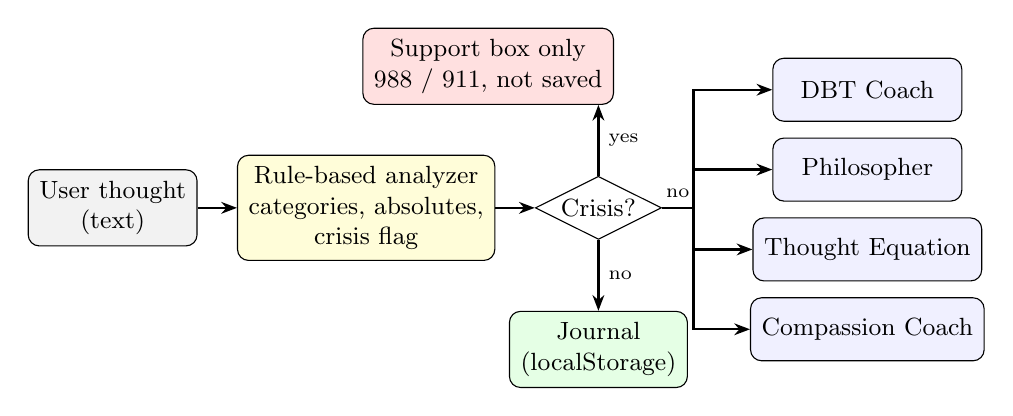
\begin{tikzpicture}[
 box/.style={draw,rounded corners,align=center,minimum height=8mm,inner sep=4pt,font=\small},
 bot/.style={box,fill=blue!6,minimum width=24mm},
 arr/.style={-{Stealth[length=2mm]},thick}]
\node[box,fill=gray!10] (in) {User thought\\(text)};
\node[box,fill=yellow!15,right=5mm of in] (an) {Rule-based analyzer\\categories, absolutes,\\crisis flag};
\node[diamond,draw,aspect=2,inner sep=1pt,font=\small,right=5mm of an] (g) {Crisis?};
\node[box,fill=red!12,above=9mm of g,xshift=-14mm] (cr) {Support box only\\988 / 911, not saved};
\node[bot,right=14mm of g,yshift=15mm] (b1) {DBT Coach};
\node[bot,below=2mm of b1] (b2) {Philosopher};
\node[bot,below=2mm of b2] (b3) {Thought Equation};
\node[bot,below=2mm of b3] (b4) {Compassion Coach};
\node[box,fill=green!10,below=9mm of g] (j) {Journal\\(localStorage)};
\draw[arr] (in)--(an); \draw[arr] (an)--(g);
\draw[arr] (g)--node[right,font=\scriptsize]{yes} (cr.south -| g);
\draw[arr] (g.east)--node[above,font=\scriptsize]{no} ++(4mm,0) |- (b1.west);
\draw[arr] (g.east)++(4mm,0) |- (b2.west);
\draw[arr] (g.east)++(4mm,0) |- (b3.west);
\draw[arr] (g.east)++(4mm,0) |- (b4.west);
\draw[arr] (g)--node[right,font=\scriptsize]{no} (j);
\end{tikzpicture}
\caption{Current MindFrame architecture. The crisis gate runs before any bot; crisis entries are neither answered with reframes nor saved.}
\label{fig:arch}
\end{figure}

\section{Proposed Framework}\label{sec:framework}
The proposal extends the prototype in five directions (Figure~\ref{fig:framework}). Each subsection states its status.

\subsection{An inner language for self-talk (speculative)}\label{sec:il}
\textbf{Idea in plain words.} The goal is to move from equations to language. Instead of only scoring a thought, MindFrame could teach a short, rhythmic way of talking to oneself, a kind of ``inner language'' with three defining features:
\begin{itemize}
\item \textbf{Time.} It is spoken slowly, with a steady rhythm, ideally paced with the breath.
\item \textbf{Silence.} Deliberate pauses are part of the language, not gaps between words. A pause is a ``word'' that means \emph{stop and notice}.
\item \textbf{A limited vocabulary.} A small set of words that are easy to remember under stress, in line with working-memory limits \citep{cowan2001}.
\end{itemize}
This combines things that already exist: DBT's STOP skill (Stop, Take a step back, Observe, Proceed mindfully), ACT defusion phrasing, mindfulness ``noting,'' and distanced self-talk \citep{kross2014}. What is new is treating them as one small \emph{grammar}. Whether such a language helps is an open, testable question.

\textbf{A small grammar.} Let the vocabulary be a set of word classes with a size cap,
\[
V = V_{\text{notice}} \cup V_{\text{name}} \cup V_{\text{stance}} \cup V_{\text{act}}, \qquad |V| \le K \;(\text{e.g., } K\approx 20),
\]
plus a family of pause tokens $\pause{d}$, where $d$ is a duration in seconds (or breaths). A minimal grammar in Backus--Naur style is:
\begin{align*}
\textit{Utterance} &\to \textit{Notice}\;\pause{d_1}\;\textit{Name}\;\pause{d_2}\;\textit{Stance}\;\pause{d_3}\;\textit{Act}\\
\textit{Notice} &\to \text{``Noticing''} \mid \text{``Here is''} \mid \text{``[own name], pause''}\\
\textit{Name} &\to \text{``a thought of''}\;C \mid \text{``a feeling of''}\;E \mid \text{``an urge to''}\;U\\
\textit{Stance} &\to \text{``that's a thought, not a fact''} \mid \text{``this is hard, and I'm not alone''}\\ &\qquad \mid \text{``not up to me''} \mid \text{``up to me''}\\
\textit{Act} &\to \text{``breathe''} \mid \text{``one small step:''}\;S \mid \text{``check the facts''} \mid \text{``opposite action''}
\end{align*}
Here $C, E, U, S$ are short slots (a category, emotion, urge, or step), each limited to a few words. An example sentence:
\begin{quote}\small
``Noticing'' $\pause{3}$ ``a thought of failure'' $\pause{3}$ ``that's a thought, not a fact'' $\pause{5}$ ``one small step: open the file.''
\end{quote}
In plain words: \emph{notice, name, take a stance, act}, with breathing room in between.

\textbf{Rhythm and silence, measured.} For an utterance with spoken duration $T_s$ and total pause duration $T_p$, define the \emph{silence ratio}
\[
\rho = \frac{T_p}{T_s + T_p}.
\]
An app could guide pacing (for instance, aiming for $\rho$ in some range such as $0.4$--$0.6$) using a visual or audio metronome. The target range is a design parameter to study, not a known optimum.

\textbf{Weighting thoughts over time.} Each journal entry $i$ has a timestamp $t_i$, a self-rated intensity $s_i\in[0,1]$, and a category vector $\mathbf{c}_i \in \{0,1\}^5$ from the analyzer. A simple exponentially decaying weight
\[
w_i(t) = s_i\, e^{-\lambda (t - t_i)}, \qquad \lambda = \frac{\ln 2}{h},
\]
with half-life $h$ (e.g., three days), gives a \emph{current thought profile}
\[
\mathbf{P}(t) = \frac{\sum_i w_i(t)\,\mathbf{c}_i}{\sum_i w_i(t)}.
\]
In plain words: recent, intense thoughts count more, and old ones fade. $\mathbf{P}(t)$ could set which skills appear first, for example leading with distress-tolerance skills when recent entries are dominated by urges. This is only a summary of what the user wrote. It is \emph{not} a diagnosis or a mood measurement.

\textbf{A better believability worksheet.} When the user actually lists evidence, a smoothed version of Eq.~\eqref{eq:b} avoids division by zero and extreme values:
\[
B' = \frac{F+1}{F+A+2}\cdot \max\bigl(0.05,\; 1-\beta D\bigr),
\]
where $F$ and $A$ are counts of user-listed facts and $\beta$ (currently $0.15$) is a tunable penalty. The ``$+1$/$+2$'' is Laplace smoothing, a standard way of starting from a neutral 50\%. The output should still be presented as a reflection aid, compared with the user's own pre/post believability rating rather than replacing it.

\subsection{An integrated self-help pipeline (partly evidence-based, integration speculative)}
Each component below has its own literature; how they are \emph{combined} is a design hypothesis. We propose a fixed, explainable sequence:
\begin{enumerate}
\item \textbf{Safety gate} (always first): crisis routing, as in the prototype.
\item \textbf{Regulate} (DBT distress tolerance, mindfulness): if intensity is high, offer STOP or TIPP before any thinking work, since examining thoughts is hard when very aroused.
\item \textbf{Notice and defuse} (ACT, inner language): put the thought into the \emph{Notice--Name--Stance} grammar.
\item \textbf{Examine} (CBT, DBT Check the Facts): evidence for and against, distortion labels, balanced rewrite.
\item \textbf{Relate kindly} (self-compassion): the three components \citep{neff2003}.
\item \textbf{Orient} (Stoicism, Frankl, ACT values): what is up to me, what matters, what stance do I choose?
\item \textbf{Act} (ACT committed action, DBT Opposite Action): one small, concrete step.
\end{enumerate}

\textbf{Grandiose ambitions.} Big dreams are not a problem in themselves, and many valuable projects start as one. The framework's aim is \emph{channeling}, not deflating: keep the value behind the dream, shrink the next step. One evidence-based technique is \emph{mental contrasting}: imagining a desired future, then the realistic obstacles, then an if--then plan. It has been found to support goal pursuit better than positive fantasy alone \citep{oettingen2014}. The pipeline would ask: \emph{What value does this dream express? What is the smallest real step this week? What obstacle is likely, and what will I do then?} At the same time, persistent, escalating grandiosity, especially with reduced need for sleep, racing thoughts, or risky behavior, can be a feature of conditions such as bipolar disorder \citep{apa2013}. A self-help app cannot tell these apart. The system should therefore offer gentle, non-alarming prompts to talk to a professional when such patterns recur (Section~\ref{sec:safety}).

\textbf{``Good or evil'' and intrusive thoughts.} Unwanted thoughts with violent, sexual, or blasphemous content are very common in the general population \citep{rachman1978}, and trying hard to suppress a thought can make it come back more often \citep{wegner1987}. Two constructive moves follow. First, \emph{defusion and normalization}: ``I'm having the thought that\ldots; many people have thoughts like this, and having a thought is not doing it.'' Second, \emph{values clarification}: the distress a person feels about a ``bad'' thought often reflects how much they care about being good. The framework should not try to argue the user out of their moral or religious commitments. It should help them act on those commitments calmly. Intrusive thoughts that are frequent, distressing, and tied to compulsive rituals can indicate OCD, which has specific effective treatments; the system should say so plainly and suggest professional support.

\textbf{Positive imagery and ``dreaming positive thoughts.''} Mental imagery has strong links to emotion, more so than verbal thought in some studies \citep{holmes2010}. The framework can offer short guided imagery: a calm place, a compassionate figure, or a vivid picture of a values-based small step completed. Following \citet{oettingen2014}, positive imagery is paired with realistic planning rather than offered as pure fantasy.

\begin{figure}[t]
\centering
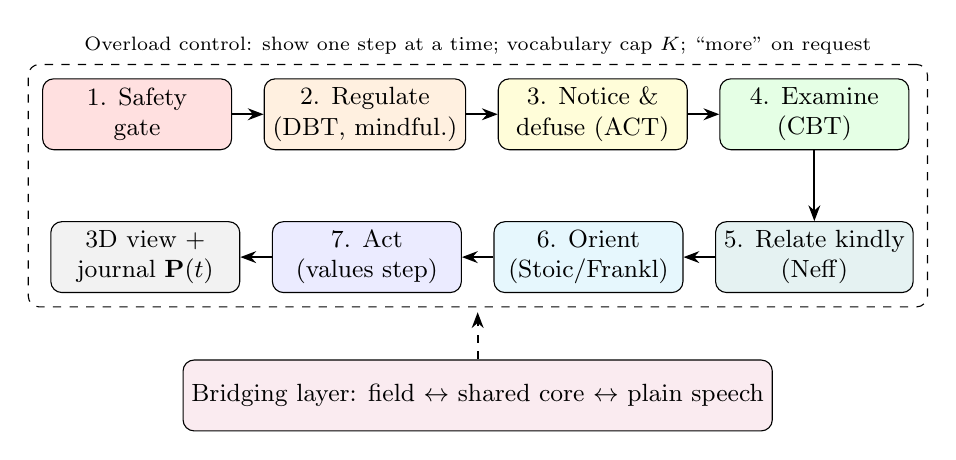
\begin{tikzpicture}[
 box/.style={draw,rounded corners,align=center,minimum width=24mm,minimum height=9mm,font=\small,inner sep=3pt},
 arr/.style={-{Stealth[length=2mm]},thick}]
\node[box,fill=red!12] (s) {1. Safety\\gate};
\node[box,fill=orange!12,right=4mm of s] (r) {2. Regulate\\(DBT, mindful.)};
\node[box,fill=yellow!15,right=4mm of r] (n) {3. Notice \&\\defuse (ACT)};
\node[box,fill=green!10,right=4mm of n] (e) {4. Examine\\(CBT)};
\node[box,fill=teal!10,below=9mm of e] (k) {5. Relate kindly\\(Neff)};
\node[box,fill=cyan!10,left=4mm of k] (o) {6. Orient\\(Stoic/Frankl)};
\node[box,fill=blue!8,left=4mm of o] (a) {7. Act\\(values step)};
\node[box,fill=gray!10,left=4mm of a] (v) {3D view +\\journal $\mathbf{P}(t)$};
\draw[arr] (s)--(r); \draw[arr] (r)--(n); \draw[arr] (n)--(e); \draw[arr] (e)--(k);
\draw[arr] (k)--(o); \draw[arr] (o)--(a); \draw[arr] (a)--(v);
\node[draw,dashed,rounded corners,fit=(s)(e)(k)(v),inner sep=5pt,label={[font=\scriptsize]above:Overload control: show one step at a time; vocabulary cap $K$; ``more'' on request}] {};
\node[box,fill=purple!8,below=13mm of $(o)!0.5!(a)$,minimum width=70mm] (b) {Bridging layer: field $\leftrightarrow$ shared core $\leftrightarrow$ plain speech};
\draw[arr,dashed] (b.north) -- ++(0,6mm);
\end{tikzpicture}
\caption{Proposed integrated framework. The order and the overload controls are design hypotheses to be tested, not validated clinical protocol.}
\label{fig:framework}
\end{figure}

\subsection{AI and 3D visualization of thought structures (design proposal)}
Two visualizations are proposed, both rendered in the browser (for example with WebGL via the three.js library):
\begin{itemize}
\item \textbf{Thought graph.} Nodes are journal entries or recurring themes. Edges connect entries that share categories. Node size reflects $w_i(t)$, so old thoughts visibly shrink and fade, a literal picture of ``thoughts pass.'' Users could drag a thought ``further away'' as an embodied defusion exercise. Any AI used here should only suggest groupings, which the user can rename or reject.
\item \textbf{Calming scene.} A slow, low-contrast 3D environment (water, sky, a path) whose motion is paced with the inner-language rhythm, for example a light that brightens on inhale and holds during pauses $\pause{d}$.
\end{itemize}
Design constraints: no flashing or fast motion (photosensitivity and arousal), an always-available ``reduce motion'' setting, a 2D fallback, and no gamified streaks or scores that could turn into pressure. Whether 3D adds anything over a simple 2D view is an empirical question; it may simply add load.

\subsection{A Langlands-inspired bridging layer (analogy, not a result)}
\textbf{What the Langlands program is.} Starting with a 1967 letter from Robert Langlands to Andr\'e Weil \citep{langlands1967}, the Langlands program is a large web of conjectures, many still open, predicting deep correspondences between number theory (in particular Galois representations, which encode symmetries of solutions to polynomial equations) and harmonic analysis/representation theory (automorphic forms and automorphic representations). Geometric versions extend the analogy to algebraic geometry. Accessible introductions include \citet{gelbart1984} and \citet{frenkel2013}, who calls it a kind of ``grand unified theory'' of mathematics. A celebrated special case of this circle of ideas, the modularity of (semistable) elliptic curves, was central to Wiles's proof of Fermat's Last Theorem \citep{wiles1995}. A proof of a major form of the geometric Langlands conjecture was announced in 2024 by a team including D.~Gaitsgory and S.~Raskin. The striking feature is that problems hard in one language become solvable once translated into another, while key quantities (such as $L$-functions) are matched across the translation.

\textbf{The design principle borrowed.} We borrow only the \emph{shape} of the idea: \emph{different fields describe shared structure in different languages; a good bridge translates while preserving what matters.} For MindFrame, the ``fields'' are DBT, CBT, ACT, self-compassion, Stoicism, and also technical domains a learner may be studying. We propose:
\begin{enumerate}
\item A \textbf{shared core vocabulary} (the inner language's word classes: notice, name, stance, act) as the common ``middle'' representation.
\item \textbf{Translation maps} from each field into the core and back, e.g., DBT ``Check the Facts'' $\mapsto$ \textsc{examine}, CBT ``evidence for/against'' $\mapsto$ \textsc{examine}, ACT ``defusion'' $\mapsto$ \textsc{stance}: thought$\neq$fact, Stoic ``dichotomy of control'' $\mapsto$ \textsc{stance}: up to me / not up to me.
\item \textbf{Invariants}: properties that must survive translation, such as the user's own meaning, the safety status, and the honesty label (evidence-based vs.\ speculative). An AI model generating a plain-speech explanation would be checked against these invariants, for example by confirming that a rephrasing does not drop a safety caveat.
\end{enumerate}
Writing $T_X: X \to \text{Core}$ for the translation of field $X$, the hope is \emph{consistency}: two fields that agree on a technique should map to the same core element, so that $T_{\text{DBT}}(\text{Check the Facts}) = T_{\text{CBT}}(\text{evidence test})$. To be explicit: \textbf{this is a metaphor and a software-design heuristic. It is not a mathematical theorem, it does not use the mathematics of the Langlands program, and it makes no claim that psychology has the rigid structure of number theory.}

\subsection{AI as a bridge without information overload (partly evidence-based)}
General-purpose AI can explain almost anything, which is exactly the risk: a distressed user, or a beginner developer learning a new field, can be buried under correct but overwhelming text. Following cognitive load theory \citep{sweller1988}, the framework proposes:
\begin{itemize}
\item \textbf{Progressive disclosure} \citep{nielsen2006}: one step of the pipeline at a time, with ``tell me more'' on request.
\item \textbf{Vocabulary cap}: responses in the default view use the core vocabulary (size $\le K$) plus at most a few new terms, each defined once.
\item \textbf{Chunk limits}: no more than about three to four options at once \citep{cowan2001}.
\item \textbf{Load-adaptive brevity}: when the profile $\mathbf{P}(t)$ or self-rated intensity is high, responses shorten further and lead with regulation skills.
\item \textbf{Grounding}: AI-generated text, if added, is constrained to a curated library of vetted skill descriptions with sources, which reduces the risk of fabricated advice \citep{bommasani2021}.
\end{itemize}


\section{The $\Psi$ Daily Reflection Index}\label{sec:psi}
The framework in Section~\ref{sec:framework} is about \emph{how} to talk to oneself. Users also benefit from a simple way to see \emph{how today is going} and which skill to try next. The $\Psi$ index serves that purpose. It is a 30-second check-in that combines five self-report terms into one number.

\begin{center}
\fbox{\begin{minipage}{0.92\linewidth}\small
\textbf{Status of $\Psi$.} $\Psi$ is a \emph{heuristic self-reflection index}. Its weights come from correlations reported in published studies on different populations and outcomes, so it has \textbf{not} been validated as a measure of anything. It must not be used to diagnose, screen for, or rule out any condition, and a high score does not mean someone is safe.
\end{minipage}}
\end{center}

\subsection{Origin: from a conceptual equation to a measurable one}
$\Psi$ began as a conceptual equation proposed by the author:
\begin{equation}
\Psi(t) = F(t)\cdot \Sigma(V) + \Lambda(C) - R(t), \qquad F(t) = \alpha e^{-\beta t} + \gamma \sin(\omega t + \phi).
\label{eq:concept}
\end{equation}
The intuition is that a person's state ($\Psi$) reflects a time-varying emotional response $F(t)$ (a decaying reaction after a trigger, plus a rhythmic component) scaled by their values $\Sigma(V)$, plus a contribution of coping $\Lambda(C)$, minus a resistance or avoidance term $R(t)$. As written, the equation cannot be computed: $\Sigma$ and $\Lambda$ are undefined operators, the terms have no units or common scale, and nothing says how to measure $V$, $C$, or $R$. We made it measurable in four steps:
\begin{enumerate}
\item \textbf{Replace undefined operators with observable quantities.} Each abstract term was mapped to a brief self-report item already close to established practice: calm (SUDS), support and belonging, skills use (diary card), avoidance (AAQ-II-style item), and thought believability (MindFrame's $B$, compared with thought-record ratings).
\item \textbf{Put everything on a common 0--1 scale}, so that each term means ``none'' at 0 and ``maximal'' at 1.
\item \textbf{Use a linear weighted sum.} A linear model is transparent, easy to explain, and hard to overfit. There is also a long-standing finding that simple linear combinations with rough weights often predict about as well as carefully fitted ones \citep{dawes1979}.
\item \textbf{Move $F(t)$ out of the daily formula} and keep it as an optional time model for how calm returns after a trigger (Section~\ref{sec:ft}), because a single daily check-in cannot estimate oscillation parameters.
\end{enumerate}

\subsection{The five measures}
\begin{table}[h]
\centering\small
\begin{tabular}{@{}l p{6.2cm} p{5.4cm}@{}}
\toprule
Term & Daily item (example wording) & Rescaling to $[0,1]$\\
\midrule
$C$ calm & ``How distressed do you feel right now?'' SUDS 0--10 & $C = 1 - \text{SUDS}/10$\\
$S$ support & ``I feel I belong and have support today'' (1--5) & $S = (x-1)/4$\\
$M$ skills & Planned coping skills for today vs.\ used (diary-card style) & $M = \text{used}/\text{planned}$ (0 if none planned)\\
$R$ avoidance & ``I avoided things I care about because of how I felt'' (1--7, adapted from AAQ-II style) & $R = (x-1)/6$\\
$B$ believability & Today's main troubling thought, worked in the Thought Equation & $B = \dfrac{F_e}{F_e + A_e}\,(1 - 0.15D)$\\
\bottomrule
\end{tabular}
\caption{The five terms of $\Psi$. $F_e$ and $A_e$ are counts of evidence for and against the thought that the user enters; $D$ is the number of detected distortions. If no evidence is entered, $F_e/(F_e+A_e)$ defaults to $0.5$ as in the prototype, and $B$ is floored at $0.05$. $B$ can be shown next to the user's own CBT-style belief rating (0--100\%) for comparison.}
\label{tab:measures}
\end{table}
Two of the five terms are proxies. SUDS measures momentary distress, so calm is assumed to be its complement. The support item is a single, untested item about belonging \citep[a construct with a long research history; see][]{baumeister1995}. The avoidance item is \emph{adapted} in the style of AAQ-II content; it is not the AAQ-II, and it has none of the AAQ-II's psychometric support.

\subsection{Deriving the weights}
Each term was matched to a published correlation between a related construct and depressive symptoms or psychopathology. Weights are the absolute correlations divided by their sum: $w_k = |r_k| / \sum_j |r_j|$.

\begin{table}[h]
\centering\small
\begin{tabular}{@{}l p{7.4cm} c c c@{}}
\toprule
Term & Source correlation used & $|r|$ & $w$ & Conservative\\
\midrule
$B$ & CFQ (cognitive fusion) with CES-D depression, $r=.85$ \citep{gillanders2014} & .85 & .308 & .267 ($|r|=.66$)\\
$R$ & AAQ-II with BDI-II, $r=.71$, $N=206$ \citep{bond2011} & .71 & .257 & .247 ($|r|=.61$)\\
$C$ & Rumination with psychopathology, meta-analytic $r=.49$ \citep{aldao2010} & .49 & .178 & .198\\
$S$ & School connectedness with depression, three-level meta-analysis of 87 studies, $r=-.39$ \citep{meng2024} & .39 & .141 & .158\\
$M$ & DBT-WCCL skills subscale with CES-D depression, $r=-.32$ (\textbf{unconfirmed}; see text) & .32 & .116 & .130\\
\midrule
 & Sum & 2.76 & 1.000 & 1.000 (sum 2.47)\\
\bottomrule
\end{tabular}
\caption{Weight derivation. Weights were rounded to two decimals for the final formula ($.18, .14, .12, .26, .31$), which sum to $1.01$.}
\label{tab:weights}
\end{table}

\paragraph{Notes on each source.}
\begin{itemize}
\item \textbf{CFQ (for $B$).} In \citet{gillanders2014}, the $r=.85$ correlation between the CFQ and the CES-D comes from a sample of 74 adults who were currently depressed, recovered, or never depressed. The authors note that the correlation was strongest in the currently depressed group, and that it was more modest ($r=.66$) in a sample of 217 dementia caregivers. We therefore treat .85 as probably inflated and use .66 in the conservative variant. The same paper notes that ``believability of thoughts'' is a narrow proxy for fusion, which is another reason the mapping from CFQ to $B$ is loose.
\item \textbf{AAQ-II (for $R$).} \citet{bond2011} report $r=.71$ between the AAQ-II and the BDI-II in a sample of 206 and $r=.70$ in a second sample. The conservative value $.61$ is the AAQ-II's correlation with DASS Depression in a sample of 432, reported in the same paper.
\item \textbf{Rumination (for $C$).} \citet{aldao2010} found a large association between rumination and psychopathology ($r=.49$). This is pooled across anxiety, depression, eating, and substance-related symptoms, not specific to depression. It is also a correlate of distress rather than of calm, so its use as the weight for $C$ is an approximation.
\item \textbf{Connectedness (for $S$).} \citet{meng2024} report $r=-.39$ between school connectedness and depression across 87 studies. The samples were students, and school connectedness is not the same as day-to-day support for adults.
\item \textbf{Skills use (for $M$).} The value $r=-.32$ between the DBT-WCCL skills subscale \citep{neacsiu2010wccl} and depressive symptoms (CES-D) was found only in a search-engine summary that appears to describe a later validation study in a partial-hospital sample. We could not confirm it from the primary article, so it is \textbf{flagged as unconfirmed} and should be checked before it is relied on. Separately, \citet{neacsiu2010mediator} found that DBT skills use mediated reductions in suicidal behavior and depression and increases in anger control during DBT, which supports including $M$ but does not provide its weight.
\end{itemize}

\paragraph{Why these weights are only a starting point.}
(1)~\emph{Different outcomes and populations}: CES-D, BDI-II, and pooled psychopathology; clinical, community, student, and caregiver samples. (2)~\emph{Collinearity and double-counting}: the CFQ and AAQ-II correlate strongly with each other ($r$ from .72 to .87 in \citealp{gillanders2014}), so $B$ and $R$ may partly count the same thing twice. (3)~\emph{Proxies}: our daily single items are not the validated scales the correlations came from. (4)~\emph{Correlation is not causation}: a strong correlation does not mean that changing the term changes mood. (5)~\emph{Bivariate, not multivariate}: normalizing zero-order correlations is not the same as estimating regression weights. These are the reasons for the personalization plan in Section~\ref{sec:personal}.

\subsection{The final equation and the Daily Score}
\begin{equation}
\boxed{\;\Psi = 0.18\,C + 0.14\,S + 0.12\,M - 0.26\,R - 0.31\,B\;}\qquad C,S,M,R,B\in[0,1].
\label{eq:psi}
\end{equation}
The smallest possible value is $-0.57$ (no calm, support, or skills; maximal avoidance and believability), and the largest is $+0.44$. The range is $1.01$, so the Daily Score
\begin{equation}
\text{Daily Score} = 100\cdot\frac{\Psi + 0.57}{1.01} \in [0, 100]
\label{eq:daily}
\end{equation}
maps the worst case to 0 and the best case to 100. In plain words: \emph{calm, support, and using skills push the score up; avoiding what matters and being hooked by a troubling thought pull it down.} The two negative terms carry the most weight because their source correlations were the largest. The conservative variant uses weights $(.198, .158, .130, -.247, -.267)$, with range $[-0.514, 0.486]$ and Daily Score $100(\Psi' + 0.514)/1.0$.

\subsection{Worked example (example values, not data)}
Suppose a user's check-in is: SUDS $=6$; support item $=4$ of 5; planned 3 skills and used 2; avoidance item $=5$ of 7; and today's thought has $F_e=2$ facts for, $A_e=3$ against, with $D=2$ distortions. \textbf{These values are invented for illustration.}

\begin{table}[h]
\centering\small
\begin{tabular}{@{}l l r r r@{}}
\toprule
Term & Computation & Value & Weight & Contribution\\
\midrule
$C$ & $1 - 6/10$ & 0.400 & $+0.18$ & $+0.072$\\
$S$ & $(4-1)/4$ & 0.750 & $+0.14$ & $+0.105$\\
$M$ & $2/3$ & 0.667 & $+0.12$ & $+0.080$\\
$R$ & $(5-1)/6$ & 0.667 & $-0.26$ & $-0.173$\\
$B$ & $\frac{2}{2+3}(1-0.15\cdot 2) = 0.4 \times 0.7$ & 0.280 & $-0.31$ & $-0.087$\\
\midrule
\multicolumn{4}{@{}l}{$\Psi$} & $-0.003$\\
\multicolumn{4}{@{}l}{Daily Score $=100(-0.003+0.57)/1.01$} & $\approx 56$\\
\bottomrule
\end{tabular}
\caption{Worked example with illustrative values. The conservative variant gives $\Psi'\approx 0.045$ and a Daily Score of $\approx 56$, so in this case the choice of weights barely matters.}
\label{tab:example}
\end{table}
\noindent To route the user to a skill, compute each term's \emph{room for improvement}: $w(1-x)$ for positive terms and $|w|\,x$ for negative terms. Here these are $C{:}\,0.108$, $S{:}\,0.035$, $M{:}\,0.040$, $R{:}\,0.173$, $B{:}\,0.087$. The largest is $R$ (avoidance), so the app would suggest \emph{Opposite Action}: one small step toward the avoided thing. If the user had rated the thought at 70\% believable on a thought record while $B=28\%$, the gap would be a useful prompt to look at the evidence again.

\subsection{Optional time model}\label{sec:ft}
The original $F(t)$ survives as an optional model of distress after a trigger at $t=0$:
\[
\text{distress}(t) = \alpha e^{-\beta t} + \gamma \sin(\omega t + \phi), \qquad C(t) = 1 - \min\bigl(1, \max(0, \text{distress}(t))\bigr).
\]
The exponential term says that distress usually fades, with half-life $\ln 2/\beta$; the sine term allows waves, such as a thought returning. This matches the common clinical observation that strong emotions rise and fall, but the specific functional form is our assumption. It could only be fitted from dense repeated ratings (e.g., EMA prompts after a trigger), and the sinusoid should be dropped unless the data clearly need it. Even the decay-only form could be useful as feedback: an illustrative message would be ``last time, your distress halved in about $X$ minutes.''

\subsection{Applications}
\begin{itemize}
\item \textbf{Daily 30-second check-in.} Five quick inputs; the Thought Equation step is optional, and $B$ is left out if skipped (with the score rescaled over the remaining weights).
\item \textbf{7-day trend.} A rolling mean of Daily Scores, shown as a gentle line, not a grade, together with the time-weighted profile $\mathbf{P}(t)$ from Section~\ref{sec:il}.
\item \textbf{Skill routing by the term with the most room for improvement}: high $B$ $\to$ Check the Facts; high $R$ $\to$ Opposite Action; low $C$ $\to$ TIPP; low $S$ $\to$ reach out to someone; low $M$ $\to$ one easy skill.
\item \textbf{Safety rule.} Any crisis language in any text field shows the crisis box (988 / 911) and suspends scoring for that entry. A sustained low score (for example, a 7-day mean below a threshold to be set conservatively) triggers a warm message encouraging the user to contact a professional or trusted person, with 988 listed. A high score never hides support options.
\end{itemize}

\begin{figure}[t]
\centering
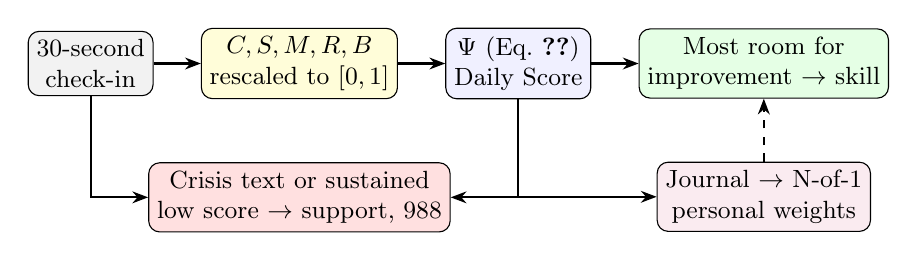
\begin{tikzpicture}[
 box/.style={draw,rounded corners,align=center,minimum height=8mm,inner sep=3pt,font=\small},
 arr/.style={-{Stealth[length=2mm]},thick}]
\node[box,fill=gray!10] (ci) {30-second\\check-in};
\node[box,fill=yellow!15,right=6mm of ci] (t) {$C,S,M,R,B$\\rescaled to $[0,1]$};
\node[box,fill=blue!6,right=6mm of t] (p) {$\Psi$ (Eq.~\ref{eq:psi})\\Daily Score};
\node[box,fill=green!10,right=6mm of p] (r) {Most room for\\improvement $\to$ skill};
\node[box,fill=red!12,below=8mm of t] (s) {Crisis text or sustained\\low score $\to$ support, 988};
\node[box,fill=purple!8,below=8mm of r] (n) {Journal $\to$ N-of-1\\personal weights};
\draw[arr] (ci)--(t); \draw[arr] (t)--(p); \draw[arr] (p)--(r);
\draw[arr] (ci) |- (s); \draw[arr] (p) |- (s);
\draw[arr] (p) |- (n); \draw[arr,dashed] (n.north) -- (r.south);
\end{tikzpicture}
\caption{How the $\Psi$ index would sit inside MindFrame. The crisis check runs on every check-in, independently of the score.}
\label{fig:psi}
\end{figure}

\subsection{Personalization}\label{sec:personal}
Literature-based weights are a starting point. Once a user has several weeks of check-ins, weights can be fitted to \emph{that user's} data, for example by regressing next-day self-rated mood on today's five terms. With few data points and correlated predictors, the fit should be regularized (e.g., ridge regression shrinking toward the literature weights), and weights should be updated slowly and shown to the user. A stronger design is an \emph{N-of-1} study \citep{kravitz2014}: alternating periods (for example, weeks with and without a daily Opposite Action step) let a single person test whether a skill actually changes their own next-day ratings, within the limits of self-report and carry-over effects.

\section{Safety and Ethics}\label{sec:safety}
\textbf{Not therapy.} MindFrame is a practice and reflection tool. It does not diagnose, treat, or replace a clinician, and it should say this in plain language on every screen, as the current safety banner does.

\textbf{Crisis routing.} The current gate puts safety before everything else and avoids the harm of ``reframing'' a suicidal statement. Its weakness is recall: keyword lists miss indirect or misspelled crisis language. Proposed improvements include broader phrase lists reviewed by clinicians, an always-visible ``I need help now'' button that does not depend on detection, localized crisis numbers outside the US, and conservative behavior under uncertainty: when in doubt, show resources. Any machine-learning classifier should be added \emph{in addition to}, never instead of, the transparent rules.

\textbf{Grandiosity, intrusive thoughts, and professional care.} As noted above, some patterns that the framework addresses (escalating grandiosity, sleeplessness with racing ideas, distressing intrusive thoughts with compulsions, persistent hopelessness) can be associated with mental health conditions \citep{apa2013}. The system should never label the user with a condition. When patterns recur in the journal, it should offer a warm, non-alarming suggestion to talk with a doctor, counselor, or trusted person.

\textbf{Respect for values and faith.} Users bring moral and religious frameworks. The tool should support users in living by their own values rather than substituting the developer's or the AI's.

\textbf{Privacy.} Journal entries are among the most sensitive data a person can write. The current design keeps them on-device in \texttt{localStorage}. Future versions should keep local-first storage as the default, add optional encryption and export, never send text to third-party AI services without explicit, informed, revocable consent, and avoid analytics on entry content. Users should be warned that \texttt{localStorage} is readable by anyone with access to the device and browser profile.

\textbf{Scores and self-worth.} A daily number can turn into a grade. The Daily Score should be framed as ``a snapshot of today's check-in,'' never as a rating of the person. It should not be gamified (no streaks, leaderboards, or rewards for high scores), and it should be easy to hide. Any threshold that triggers a support message should err on the side of offering help.

\textbf{Over-trust.} The ``ELIZA effect'' \citep{weizenbaum1966} warns that users may credit simple programs with understanding. Bots should be labeled as templates or AI, and numbers like $B$ and $\Psi$ should be labeled as heuristics.

\section{Evaluation Plan}\label{sec:eval}
\textbf{No studies have been run, and no results are reported here.} We propose a staged plan; any study involving human participants would require ethics review (e.g., an Institutional Review Board), informed consent, and a crisis protocol.
\begin{enumerate}
\item \textbf{Technical evaluation of the analyzer.} Build a labeled test set of short sentences, including tricky cases (negations, misspellings, the \texttt{sin} false-positive class such as ``cousin'', indirect crisis language). Report precision and recall per category, with priority on crisis \emph{recall}. This can be done without human participants by using synthetic and publicly available examples.
\item \textbf{Usability study} (small $n$, non-clinical adult volunteers). Measures: task completion, the System Usability Scale, and perceived workload (e.g., NASA-TLX), comparing a full-text view against the progressive-disclosure view.
\item \textbf{Inner-language feasibility.} Can participants learn and recall the grammar after one session and after one week? Do they find pauses helpful or awkward? Mixed methods: recall tests plus interviews.
\item \textbf{Single-session pilot.} Within-subject pre/post ratings of believability of a self-chosen negative thought and of momentary distress, with an active comparison (e.g., free journaling). Established self-report scales (such as Neff's Self-Compassion Scale) could be used as secondary measures over longer studies.
\item \textbf{Visualization comparison.} 2D list vs.\ 2D graph vs.\ 3D scene on perceived calm, load, and preference, with motion-sensitivity screening.
\item \textbf{$\Psi$ measurement study.} With consenting adult volunteers doing daily check-ins for several weeks: test--retest stability of each item on repeated same-day ratings; within-person correlations between the Daily Score and a weekly established measure such as the PHQ-8 \citep{kroenke2009}, chosen because it omits the suicidality item and so does not need in-app risk follow-up (crisis routing still applies); and comparison of the literature weights, the conservative weights, equal weights \citep{dawes1979}, and personally fitted weights in predicting next-day mood on held-out days.
\item \textbf{Believability comparison.} Agreement between MindFrame's $B$ and users' own thought-record belief ratings (0--100\%), before and after the worksheet.
\item \textbf{Skill-routing usefulness.} Whether users rate the suggested skill as more relevant than a random skill, in a blinded within-person comparison.
\item \textbf{Bridging layer audit.} For AI-generated plain-speech translations, have expert raters judge whether invariants (meaning, safety caveats, evidence labels) were preserved.
\end{enumerate}
Even positive pilot results would show only short-term feasibility and acceptability, not clinical efficacy. Efficacy would require larger randomized trials conducted with clinical researchers.

\section{Limitations}
The prototype's analyzer is shallow and English-only; its believability score is arbitrary; the bots are templates that do not adapt to context. The proposed framework combines traditions that have different theoretical assumptions (for example, CBT challenges thought content, while ACT emphasizes changing one's relationship to thoughts rather than their content), and a fixed pipeline may smooth over real disagreements. The inner language is untested and may feel artificial. The linguistic-relativity motivation rests on its weaker, contested forms. The Langlands analogy could mislead readers into thinking the framework has mathematical backing; we have tried to prevent this by labeling it clearly. The $\Psi$ index adds its own limits: its weights come from studies of different constructs, outcomes, and populations; two inputs are proxies; $B$ and $R$ probably overlap; one weight rests on an unconfirmed correlation; and a single daily number compresses a great deal. Finally, the author is a beginner developer, not a clinician or mathematician, and expert review is needed throughout.

\section{Future Work}
Near-term fixes to the prototype: add a leading word boundary to the \texttt{sin} pattern and handle negation; let users enter real evidence so that $B$ uses actual counts; add an always-on help button and international crisis numbers. Medium-term: implement the Notice--Name--Stance--Act grammar as a guided, paced exercise; a 2D thought graph with decaying weights and then an optional 3D calming scene; and a curated, cited skills library as the grounding source for any AI. Longer-term: the field-to-core translation tables, extending the bridge to technical learning (for example, explaining programming concepts in the same limited, paced style), clinician co-design, and confirmation of the DBT-WCCL correlation from the primary source. The most important next step, which ties these together, is described in Section~\ref{sec:next}.

\section{Conclusion}
MindFrame shows that a small, transparent tool can bring several evidence-based self-help traditions into one place while putting safety first. This paper proposes a path from that prototype toward a more unified framework: a paced, quiet, limited-vocabulary inner language; an ordered pipeline from regulation to values-based action; visualizations in which thoughts visibly pass; a bridge between fields, inspired by the Langlands program only as a metaphor, that translates into plain speech without overwhelming the user; and the $\Psi$ index, a measurable descendant of an intuitive equation that turns a daily check-in into a gentle score and a suggested skill. Each piece is offered as a hypothesis to be tested carefully, with humility about what a self-help app can and cannot do.

\section{Next Project: MindFrame $\Psi$-Lab}\label{sec:next}
\textbf{One-sentence pitch.} \emph{MindFrame $\Psi$-Lab} is a privacy-first extension of MindFrame that pairs a daily $\Psi$ check-in with a short inner-language practice and lets each user, and eventually a small consented study, test whether the practice and the routed skills actually help that person, using an N-of-1 design.

\subsection{Goals}
\begin{enumerate}
\item \textbf{Unify the two halves of this paper}: the inner language (\emph{how} to talk to oneself) and $\Psi$ (\emph{how today is going} and \emph{what to try next}) in one daily flow of about two minutes.
\item \textbf{Make the claims testable}: replace literature weights with evidence about each user, and find out whether inner-language practice is feasible and acceptable.
\item \textbf{Keep the safety and privacy guarantees} of the current prototype: crisis-first routing, local-first storage, and no hidden data collection.
\item \textbf{Stay a beginner-friendly codebase}: static site, plain JavaScript, readable math, and tests.
\end{enumerate}

\subsection{MVP feature list}
\begin{enumerate}
\item \textbf{Check-in screen}: SUDS slider, support item, planned/used skills checklist, avoidance item, optional Thought Equation with real $F_e$/$A_e$ entry; computes $C,S,M,R,B$, $\Psi$, and the Daily Score, with a ``how this was calculated'' panel.
\item \textbf{Crisis gate on every text field}, with the analyzer's \texttt{sin} fix and negation handling, an always-visible help button, and 988/911.
\item \textbf{Inner-language practice}: a guided Notice $\pause{}$ Name $\pause{}$ Stance $\pause{}$ Act sequence with a breathing-paced visual metronome and an adjustable silence ratio $\rho$.
\item \textbf{Skill routing} by the term with the most room for improvement, showing one skill at a time (progressive disclosure).
\item \textbf{7-day trend view} in 2D (Daily Score line plus a small bar for each term), with a sustained-low-score support message.
\item \textbf{Weight switcher}: literature, conservative, and equal weights, plus personal weights once enough data exist.
\item \textbf{N-of-1 mode}: the user picks one skill (e.g., Opposite Action) and the app schedules alternating ``with'' and ``without'' weeks, then shows a simple comparison with uncertainty.
\item \textbf{Local-first data}: \texttt{localStorage} or IndexedDB, CSV/JSON export, one-tap delete, no analytics on content.
\item \textbf{Unit tests} for every formula (rescaling, $B$, $\Psi$, Daily Score bounds, routing).
\end{enumerate}

\subsection{Milestones}
\begin{table}[h]
\centering\small
\begin{tabular}{@{}l p{11.8cm}@{}}
\toprule
Milestone & Deliverable\\
\midrule
M1 (weeks 1--2) & Analyzer fixes, crisis-gate tests, formula module with unit tests (bounds: score always in $[0,100]$).\\
M2 (weeks 3--4) & Check-in screen, Daily Score, ``how calculated'' panel, skill routing.\\
M3 (weeks 5--6) & Inner-language guided practice with pacing; 7-day trend view; export/delete.\\
M4 (weeks 7--8) & Weight switcher, personal-weight fitting (ridge toward literature weights), N-of-1 scheduler and summary.\\
M5 (weeks 9--12) & Author self-use pilot (an N-of-1 with oneself, not a study); expert feedback from a clinician on safety copy; fix issues.\\
M6 (later) & If a clinical or academic collaborator and ethics approval are available: the small consented study from Section~\ref{sec:eval}.\\
\bottomrule
\end{tabular}
\caption{Proposed milestones. Durations are planning estimates for a part-time beginner developer.}
\end{table}

\subsection{How success would be measured}
Success criteria are set \emph{before} any data exist, so that results cannot be cherry-picked. None of these have been measured.
\begin{itemize}
\item \textbf{Engineering}: all formula tests pass; crisis-gate recall on the labeled test set is reported, with every missed crisis example fixed or documented; no network requests carry journal content.
\item \textbf{Feasibility}: proportion of days with a completed check-in over four weeks, and median check-in time (target around two minutes or less).
\item \textbf{Acceptability}: usability ratings and short interviews on whether the score feels helpful or judgmental, and whether pauses feel calming or awkward.
\item \textbf{Measurement}: whether the Daily Score tracks weekly PHQ-8 scores within persons, and whether personal weights predict held-out next-day mood better than literature or equal weights.
\item \textbf{Usefulness}: whether routed skills are rated more relevant than random ones, and, in N-of-1 mode, whether a chosen skill is associated with higher next-day ratings for that person (reported with uncertainty, not as proof).
\item \textbf{Safety}: zero instances of a crisis entry receiving bot output; every sustained-low-score episode shows the support message.
\end{itemize}
A null or negative result on any of these would also be a valuable, publishable outcome. It would tell us which parts of the framework to simplify or drop.

\begin{thebibliography}{99}\small
\setlength{\itemsep}{1pt}
\bibitem[{Aldao et~al.(2010)}]{aldao2010} Aldao, A., Nolen-Hoeksema, S., \& Schweizer, S. (2010). Emotion-regulation strategies across psychopathology: A meta-analytic review. \emph{Clinical Psychology Review, 30}(2), 217--237.
\bibitem[{Alderson-Day and Fernyhough(2015)}]{aldersonday2015} Alderson-Day, B., \& Fernyhough, C. (2015). Inner speech: Development, cognitive functions, phenomenology, and neurobiology. \emph{Psychological Bulletin, 141}(5), 931--965.
\bibitem[{American Psychiatric Association(2013)}]{apa2013} American Psychiatric Association. (2013). \emph{Diagnostic and Statistical Manual of Mental Disorders} (5th ed.). Arlington, VA: APA.
\bibitem[{Baumeister and Leary(1995)}]{baumeister1995} Baumeister, R. F., \& Leary, M. R. (1995). The need to belong: Desire for interpersonal attachments as a fundamental human motivation. \emph{Psychological Bulletin, 117}(3), 497--529.
\bibitem[{Beck(1976)}]{beck1976} Beck, A. T. (1976). \emph{Cognitive Therapy and the Emotional Disorders}. New York: International Universities Press.
\bibitem[{Beck et~al.(1979)}]{beck1979} Beck, A. T., Rush, A. J., Shaw, B. F., \& Emery, G. (1979). \emph{Cognitive Therapy of Depression}. New York: Guilford Press.
\bibitem[{Beck(2011)}]{beck2011} Beck, J. S. (2011). \emph{Cognitive Behavior Therapy: Basics and Beyond} (2nd ed.). New York: Guilford Press.
\bibitem[{Bommasani et~al.(2021)}]{bommasani2021} Bommasani, R., et al. (2021). On the opportunities and risks of foundation models. \emph{arXiv preprint} arXiv:2108.07258.
\bibitem[{Bond et~al.(2011)}]{bond2011} Bond, F. W., Hayes, S. C., Baer, R. A., Carpenter, K. M., Guenole, N., Orcutt, H. K., Waltz, T., \& Zettle, R. D. (2011). Preliminary psychometric properties of the Acceptance and Action Questionnaire--II: A revised measure of psychological inflexibility and experiential avoidance. \emph{Behavior Therapy, 42}(4), 676--688.
\bibitem[{Boroditsky(2001)}]{boroditsky2001} Boroditsky, L. (2001). Does language shape thought? Mandarin and English speakers' conceptions of time. \emph{Cognitive Psychology, 43}(1), 1--22.
\bibitem[{Burns(1980)}]{burns1980} Burns, D. D. (1980). \emph{Feeling Good: The New Mood Therapy}. New York: William Morrow.
\bibitem[{Cowan(2001)}]{cowan2001} Cowan, N. (2001). The magical number 4 in short-term memory: A reconsideration of mental storage capacity. \emph{Behavioral and Brain Sciences, 24}(1), 87--114.
\bibitem[{Dawes(1979)}]{dawes1979} Dawes, R. M. (1979). The robust beauty of improper linear models in decision making. \emph{American Psychologist, 34}(7), 571--582.
\bibitem[{Epictetus(c.~125)}]{epictetus} Epictetus. (c.~125 CE). \emph{Enchiridion} (Handbook). Various translations.
\bibitem[{Fernyhough(2016)}]{fernyhough2016} Fernyhough, C. (2016). \emph{The Voices Within: The History and Science of How We Talk to Ourselves}. New York: Basic Books.
\bibitem[{Fitzpatrick et~al.(2017)}]{fitzpatrick2017} Fitzpatrick, K. K., Darcy, A., \& Vierhile, M. (2017). Delivering cognitive behavior therapy to young adults with symptoms of depression and anxiety using a fully automated conversational agent (Woebot): A randomized controlled trial. \emph{JMIR Mental Health, 4}(2), e19.
\bibitem[{Frankl(1946/2006)}]{frankl2006} Frankl, V. E. (2006). \emph{Man's Search for Meaning}. Boston: Beacon Press. (Original work published 1946.)
\bibitem[{Frenkel(2013)}]{frenkel2013} Frenkel, E. (2013). \emph{Love and Math: The Heart of Hidden Reality}. New York: Basic Books.
\bibitem[{Gelbart(1984)}]{gelbart1984} Gelbart, S. (1984). An elementary introduction to the Langlands program. \emph{Bulletin of the American Mathematical Society, 10}(2), 177--219.
\bibitem[{Gillanders et~al.(2014)}]{gillanders2014} Gillanders, D. T., Bolderston, H., Bond, F. W., Dempster, M., Flaxman, P. E., Campbell, L., \ldots\ Remington, B. (2014). The development and initial validation of the Cognitive Fusion Questionnaire. \emph{Behavior Therapy, 45}(1), 83--101. Author version: \url{https://www.pure.ed.ac.uk/ws/files/15143836/Gillanders_et_al_2014.pdf}
\bibitem[{Hayes et~al.(2012)}]{hayes2012} Hayes, S. C., Strosahl, K. D., \& Wilson, K. G. (2012). \emph{Acceptance and Commitment Therapy: The Process and Practice of Mindful Change} (2nd ed.). New York: Guilford Press.
\bibitem[{Hofmann et~al.(2012)}]{hofmann2012} Hofmann, S. G., Asnaani, A., Vonk, I. J. J., Sawyer, A. T., \& Fang, A. (2012). The efficacy of cognitive behavioral therapy: A review of meta-analyses. \emph{Cognitive Therapy and Research, 36}(5), 427--440.
\bibitem[{Holmes and Mathews(2010)}]{holmes2010} Holmes, E. A., \& Mathews, A. (2010). Mental imagery in emotion and emotional disorders. \emph{Clinical Psychology Review, 30}(3), 349--362.
\bibitem[{Kabat-Zinn(1990)}]{kabatzinn1990} Kabat-Zinn, J. (1990). \emph{Full Catastrophe Living}. New York: Delacorte.
\bibitem[{Kravitz et~al.(2014)}]{kravitz2014} Kravitz, R. L., Duan, N., \& the DEcIDE Methods Center N-of-1 Guidance Panel (Eds.). (2014). \emph{Design and Implementation of N-of-1 Trials: A User's Guide}. Rockville, MD: Agency for Healthcare Research and Quality.
\bibitem[{Kroenke et~al.(2009)}]{kroenke2009} Kroenke, K., Strine, T. W., Spitzer, R. L., Williams, J. B. W., Berry, J. T., \& Mokdad, A. H. (2009). The PHQ-8 as a measure of current depression in the general population. \emph{Journal of Affective Disorders, 114}(1--3), 163--173.
\bibitem[{Kross et~al.(2014)}]{kross2014} Kross, E., Bruehlman-Senecal, E., Park, J., et al. (2014). Self-talk as a regulatory mechanism: How you do it matters. \emph{Journal of Personality and Social Psychology, 106}(2), 304--324.
\bibitem[{Langlands(1967)}]{langlands1967} Langlands, R. P. (1967). Letter to Andr\'e Weil. (Available via the Institute for Advanced Study's Langlands archive.)
\bibitem[{Linehan(1993)}]{linehan1993} Linehan, M. M. (1993). \emph{Cognitive-Behavioral Treatment of Borderline Personality Disorder}. New York: Guilford Press.
\bibitem[{Linehan(2015)}]{linehan2015} Linehan, M. M. (2015). \emph{DBT Skills Training Manual} (2nd ed.). New York: Guilford Press.
\bibitem[{Marcus Aurelius(c.~180)}]{marcus} Marcus Aurelius. (c.~170--180 CE). \emph{Meditations}. Various translations.
\bibitem[{Meng et~al.(2024)}]{meng2024} Meng, X., Chen, Y., Wang, X., Yuan, J., \& Yu, D. (2024). The relationship between school connectedness and depression: A three-level meta-analytic review. \emph{Advances in Psychological Science, 32}(2), 246--263. (In Chinese with English abstract.)
\bibitem[{Miller(1956)}]{miller1956} Miller, G. A. (1956). The magical number seven, plus or minus two: Some limits on our capacity for processing information. \emph{Psychological Review, 63}(2), 81--97.
\bibitem[{Neacsiu et~al.(2010a)}]{neacsiu2010mediator} Neacsiu, A. D., Rizvi, S. L., \& Linehan, M. M. (2010). Dialectical behavior therapy skills use as a mediator and outcome of treatment for borderline personality disorder. \emph{Behaviour Research and Therapy, 48}(9), 832--839.
\bibitem[{Neacsiu et~al.(2010b)}]{neacsiu2010wccl} Neacsiu, A. D., Rizvi, S. L., Vitaliano, P. P., Lynch, T. R., \& Linehan, M. M. (2010). The Dialectical Behavior Therapy Ways of Coping Checklist: Development and psychometric properties. \emph{Journal of Clinical Psychology, 66}(6), 563--582.
\bibitem[{Neff(2003)}]{neff2003} Neff, K. D. (2003). Self-compassion: An alternative conceptualization of a healthy attitude toward oneself. \emph{Self and Identity, 2}(2), 85--101.
\bibitem[{Nielsen(2006)}]{nielsen2006} Nielsen, J. (2006). Progressive disclosure. Nielsen Norman Group article, nngroup.com.
\bibitem[{Oettingen(2014)}]{oettingen2014} Oettingen, G. (2014). \emph{Rethinking Positive Thinking: Inside the New Science of Motivation}. New York: Current.
\bibitem[{Rachman and de Silva(1978)}]{rachman1978} Rachman, S., \& de Silva, P. (1978). Abnormal and normal obsessions. \emph{Behaviour Research and Therapy, 16}(4), 233--248.
\bibitem[{Robertson(2010)}]{robertson2010} Robertson, D. (2010). \emph{The Philosophy of Cognitive-Behavioural Therapy (CBT): Stoic Philosophy as Rational and Cognitive Psychotherapy}. London: Karnac.
\bibitem[{Shiffman et~al.(2008)}]{shiffman2008} Shiffman, S., Stone, A. A., \& Hufford, M. R. (2008). Ecological momentary assessment. \emph{Annual Review of Clinical Psychology, 4}, 1--32.
\bibitem[{Sweller(1988)}]{sweller1988} Sweller, J. (1988). Cognitive load during problem solving: Effects on learning. \emph{Cognitive Science, 12}(2), 257--285.
\bibitem[{Vygotsky(1934/1986)}]{vygotsky1986} Vygotsky, L. S. (1986). \emph{Thought and Language} (A. Kozulin, Ed. \& Trans.). Cambridge, MA: MIT Press. (Original work published 1934.)
\bibitem[{Wegner et~al.(1987)}]{wegner1987} Wegner, D. M., Schneider, D. J., Carter, S. R., \& White, T. L. (1987). Paradoxical effects of thought suppression. \emph{Journal of Personality and Social Psychology, 53}(1), 5--13.
\bibitem[{Weizenbaum(1966)}]{weizenbaum1966} Weizenbaum, J. (1966). ELIZA---A computer program for the study of natural language communication between man and machine. \emph{Communications of the ACM, 9}(1), 36--45.
\bibitem[{Whorf(1956)}]{whorf1956} Whorf, B. L. (1956). \emph{Language, Thought, and Reality} (J. B. Carroll, Ed.). Cambridge, MA: MIT Press.
\bibitem[{Wiles(1995)}]{wiles1995} Wiles, A. (1995). Modular elliptic curves and Fermat's Last Theorem. \emph{Annals of Mathematics, 141}(3), 443--551.
\bibitem[{Wolpe(1969)}]{wolpe1969} Wolpe, J. (1969). \emph{The Practice of Behavior Therapy}. New York: Pergamon Press.
\end{thebibliography}
\end{document}
